% This is samplepaper.tex, a sample chapter demonstrating the
% LLNCS macro package for Springer Computer Science proceedings;
% Version 2.20 of 2017/10/04
%
\documentclass[runningheads]{llncs}
%
\usepackage{graphicx}
\usepackage{latexsym}
\usepackage{algorithm}
\usepackage{algorithmic}
\usepackage{setspace}

% Used for displaying a sample figure. If possible, figure files should
% be included in EPS format.
%
% If you use the hyperref package, please uncomment the following line
% to display URLs in blue roman font according to Springer's eBook style:
% \renewcommand\UrlFont{\color{blue}\rmfamily}

\begin{document}

%
\title{Multiple Question Answer Optimization in RDF Q/A System\thanks{Supported by organization x.}}
\author{}
\institute{}
%
%\titlerunning{Abbreviated paper title}
% If the paper title is too long for the running head, you can set
% an abbreviated paper title here
%
%
\maketitle              % typeset the header of the contribution
%
\begin{abstract}
RDF Question/Answer(Q/A) system allows users to ask questions in natural languages over Knowledge Graph represented by RDF. To answer a natural language question, a lot of excellent work has been done. However, existing work on RDF Q/A mainly focuses on a-question-at-a-time approaches. When multiple questions arrive at the same time, sequential processing is not always the most efficient. In this paper, We first propose a novel approach for efficiently detecting useful semantic information in natural language. Then we give a way to improve the efficiency of the RDF Q/A system by using the common semantic parts. Experiment confirm that our method not only keeps the precision but also speeds up query performance greatly.
\keywords{Multiple-Question  \and Knowledge Graph \and RDF Q/A.}
\end{abstract}
%
%
%
\section{Introduction}

Knowledge Graph(KG) has become a very popular way to represent and query world knowledge. RDF and SPARQL are two core concepts in the Knowledge Graph, which are standards for representing and querying Knowledge Graph, recommended by the W3C. Although SPARQL is a standard way to access RDF data, it remains tedious and difficult for users. Hence, qustion/answering(Q/A) based on Knowledge Graph has received wide attention in both natural language processing and database areas.

Generally, there are two significant challenges in RDF Q/A systems:\textit{\textbf{question understanding}}(Question $\rightarrow$ SPARQL) and \textit{\textbf{query evaluation}}. A great deal of research has been done to address the first challenge. For example, Zou et al\cite{gAnswer}. proposed two frameworks to build the semantic query graph. To overcome the second challenge, single-machine RDF systems, like RDF-3X\cite{RDF3X},gStore\cite{gStore} and many distributed SPARQL query engines have been introduced.

However, in some scenarios multiple queries can be processed as a batch. For example, in Q/A system, multiple questions often need to be processed together. Therefore, the third challenge arises in RDF Q/A system: "How can RDF Q/A System handle batch questions efficiently". Some research work has been proposed to efficiently process multiple SPARQL queries\cite{junhu}. However, efficient processing of multiple SPARQL queries is not equivalent to multiple Question Answer. Because  batch processing of SPARQL queries is only part of the second challenge.

The main contribution of this paper is an effective solution to the multiple questions answer optimization in RDF Q/A system.

\section{Overview of Our Approach}
The main contribution of this paper is an effective solution to the multiple Question Answer optimization problem in RDF Q/A System. Specifically,
\begin{enumerate}
	\item By searching and utilizing the common structure in the Question undestanding stage, the system efficiency is improved.
	\item How to measure the core degree of words in a natual language question for generating SPARQL queries is given.
\end{enumerate}
\subsection{Detecting Common Structure}
\begin{figure}
	\centering
	\label{process}
	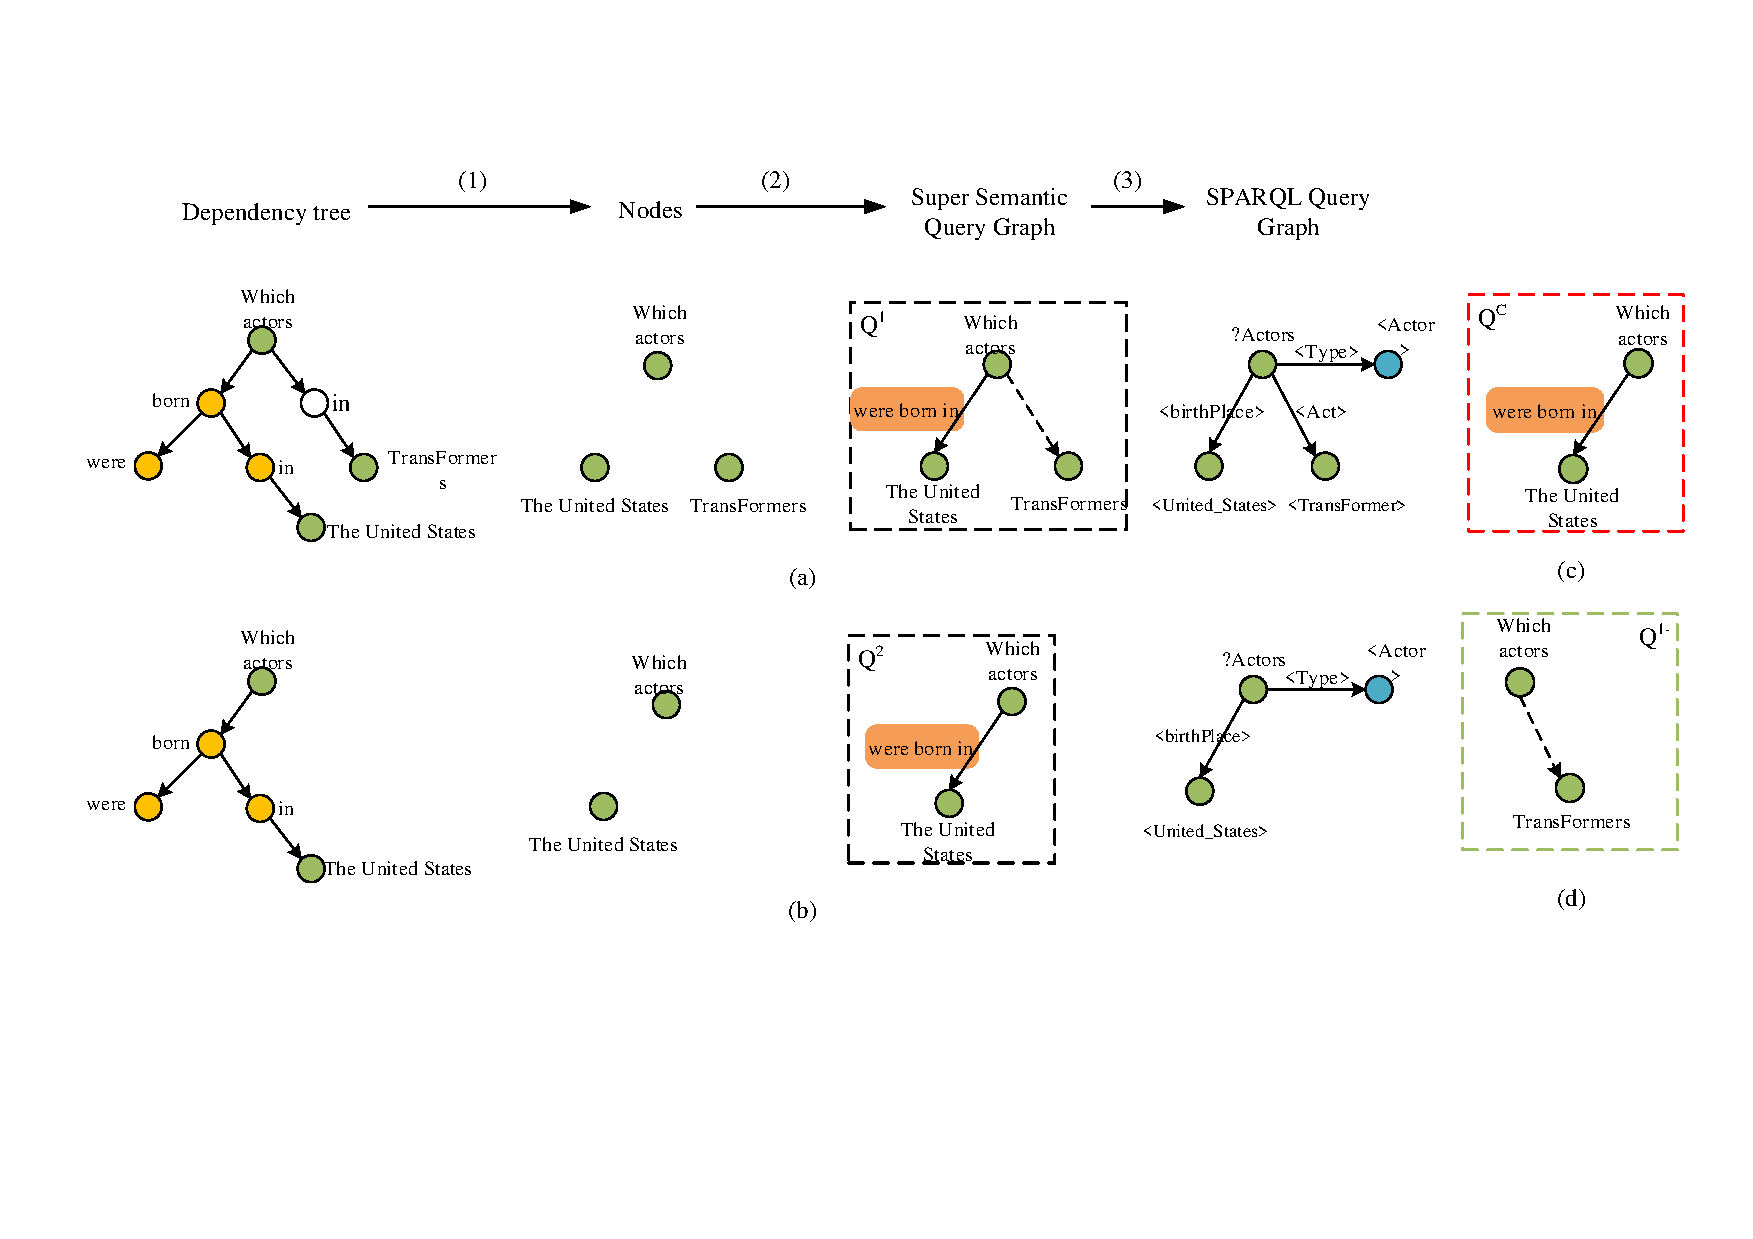
\includegraphics[width=\textwidth]{process.pdf}
	\caption{Acceleration Ratio}
\end{figure}
Figure 1 (a) shows a process of transforming question ``\textit{Which actors in Transformers were born in the United States?}" into a SPARQL query graph. The first step is to recognize all nodes from the question sentence N.(1) Generally, we extract entities, classes and wild-cards as nodes. We adopt the dictionary-based entity linking approach [5] to find entities and classes. Given a node set V (which has been recognized in the first step) and a dependency tree Y of question sentence, for any two nodes $v_{i}$ and $v_{j}(\in V)$, we introduce an edge between $v_{i}$ and $v_{j}$ if and only if the simple path between $v_{i}$ and $v_{j}$ does not contain other node in V. Finally, the phrases linking operation is executed.

Assuming that there are two questions $N_{1}$(``\textit{Which actors in Transformers were born in the United States?}") and $N_{2}$(``\textit{Which actors were born in the United States?}") to be processed by RDF Q/A system, Figure 1 (a) shows the process of question $N_{1}$ and Figure 1 (b) shows the process of $N_{2}$. We can see that there is a common structure $Q^{C}$(Figure 1(c)) between Super Semantic Query Graph generated in (a) and (b). We can take this common part out to execute Phrases Linking separately, and then question $N_{1}$ only needs to execute Phrases Linking operation on $Q_{1}^{-}$(Figure 1(d)) part.
\subsection{Semantic Capture}
In the challenge of Question Understanding, we tried to use the SPARQL \textit{Q} to accurately express the semantics of the question \textit{N}. In fact, the different words in \textit{N} are different in the importance of generating \textit{Q}. However, there is currently no way to measure the importance of each word in \textit{N} for generating \textit{Q}. Question Understanding can be expressed by the following formula:$f(N) \rightarrow Q$. 

The natural language question N is composed of the word $w_{i}$, and the SPARQL is composed of triple pattern $t_{j}$, so that we can convert the $f(N) \rightarrow Q$ into $f(w_{1},w_{2},...,w_{n})=(t_{1},t_{2},...t_{m})$, and then by vectorizing $w_{i}$ and $t_{j}$ we can get the following formula:
\begin{equation}
\label{e2}
f(\overrightarrow{w_{1}},\overrightarrow{w_{2}},...,\overrightarrow{w_{n}}) \rightarrow (\overrightarrow{t_{1}},\overrightarrow{t_{2}},...,\overrightarrow{t_{m}})
\end{equation}
we defined a loss function as follows.
\begin{equation}
\label{e6}
L =\sum_{}^{} (\sum_{i=1}^{m}\overrightarrow{t_{i}}-\sum_{j=1}^{n}\overrightarrow{w_{i}})
\end{equation}
By Equation 3, we make the overall $\langle N_{i}, Q_{j} \rangle$ in the data set as equal as possible. That is, $(\overrightarrow{w_{1}}+\overrightarrow{w_{2}}+...+\overrightarrow{w_{n}}) = (\overrightarrow{t_{1}}+\overrightarrow{t_{2}}+...+\overrightarrow{t_{m}})$. So we give each $w_{i}$ a suitable vector representation. Then we can use the following formula to measure the core of a word $w_{i}$ in N.
\begin{equation}
\label{e7}
\omega = \frac{\sum_{j=1}^{m}w_{i}^{j}}{\sum_{i=1}^{n} \sum_{j=1}^{m}w_{i}^{j}}
\end{equation}
Where $w_{i}^{j}$ represents the value of the vector $w_{i}$ in the jth dimension.

With the method of getting the core degree of each word $w_{i}$ in N, we need to consider how to get a large enough $\langle  Question, Query \rangle$ data set, that is, how to get a SPARQL Query Q corresponding to Natual Language N correctly.
We chose to use gAnswer to generate a SPARQL Q for each question in the $\langle Question, Answer \rangle$ dataset(SQuAD). If Q returns the same result as Answer on the data set, the $\langle Question, Query \rangle$ pair is retained. Then we get a large enough $\langle Question, Query \rangle$ data set.
\section{Experiment and Evaluation}
\begin{table}
	\centering
	\label{table1}
	\caption{Evaluating QALD Testing Questions.}
\begin{tabular}{cccccc}
	\hline
	& Processed& Right& Recall& Precision&F-1\\
	\hline  %添加表格中横线
	\textbf{Our Approach} &100 &70 & 0.74& 0.90& 0.80\\
	gAnswer &100 &68 & 0.72& 0.89& 0.78\\
	RFF &100 &40 & 0.43& 0.77& 0.55\\
	KWGAnswer &100 &52 & 0.59& 0.85& 0.70\\
	Aqqu &100 &36 & 0.37& 0.39& 0.38\\
	\hline %添加表格底部粗线
\end{tabular}
\end{table}
From the data shown in Table 1, we can see that the accuracy of Our Approach is slightly higher than the original paper gAnswer because of the better selection of words $w_{i}$ in natural language problem N (filtering out some possible interference information).
\begin{figure}
	\centering
	\begin{minipage}[t]{0.48\textwidth}
		\centering
		\label{fig2}
		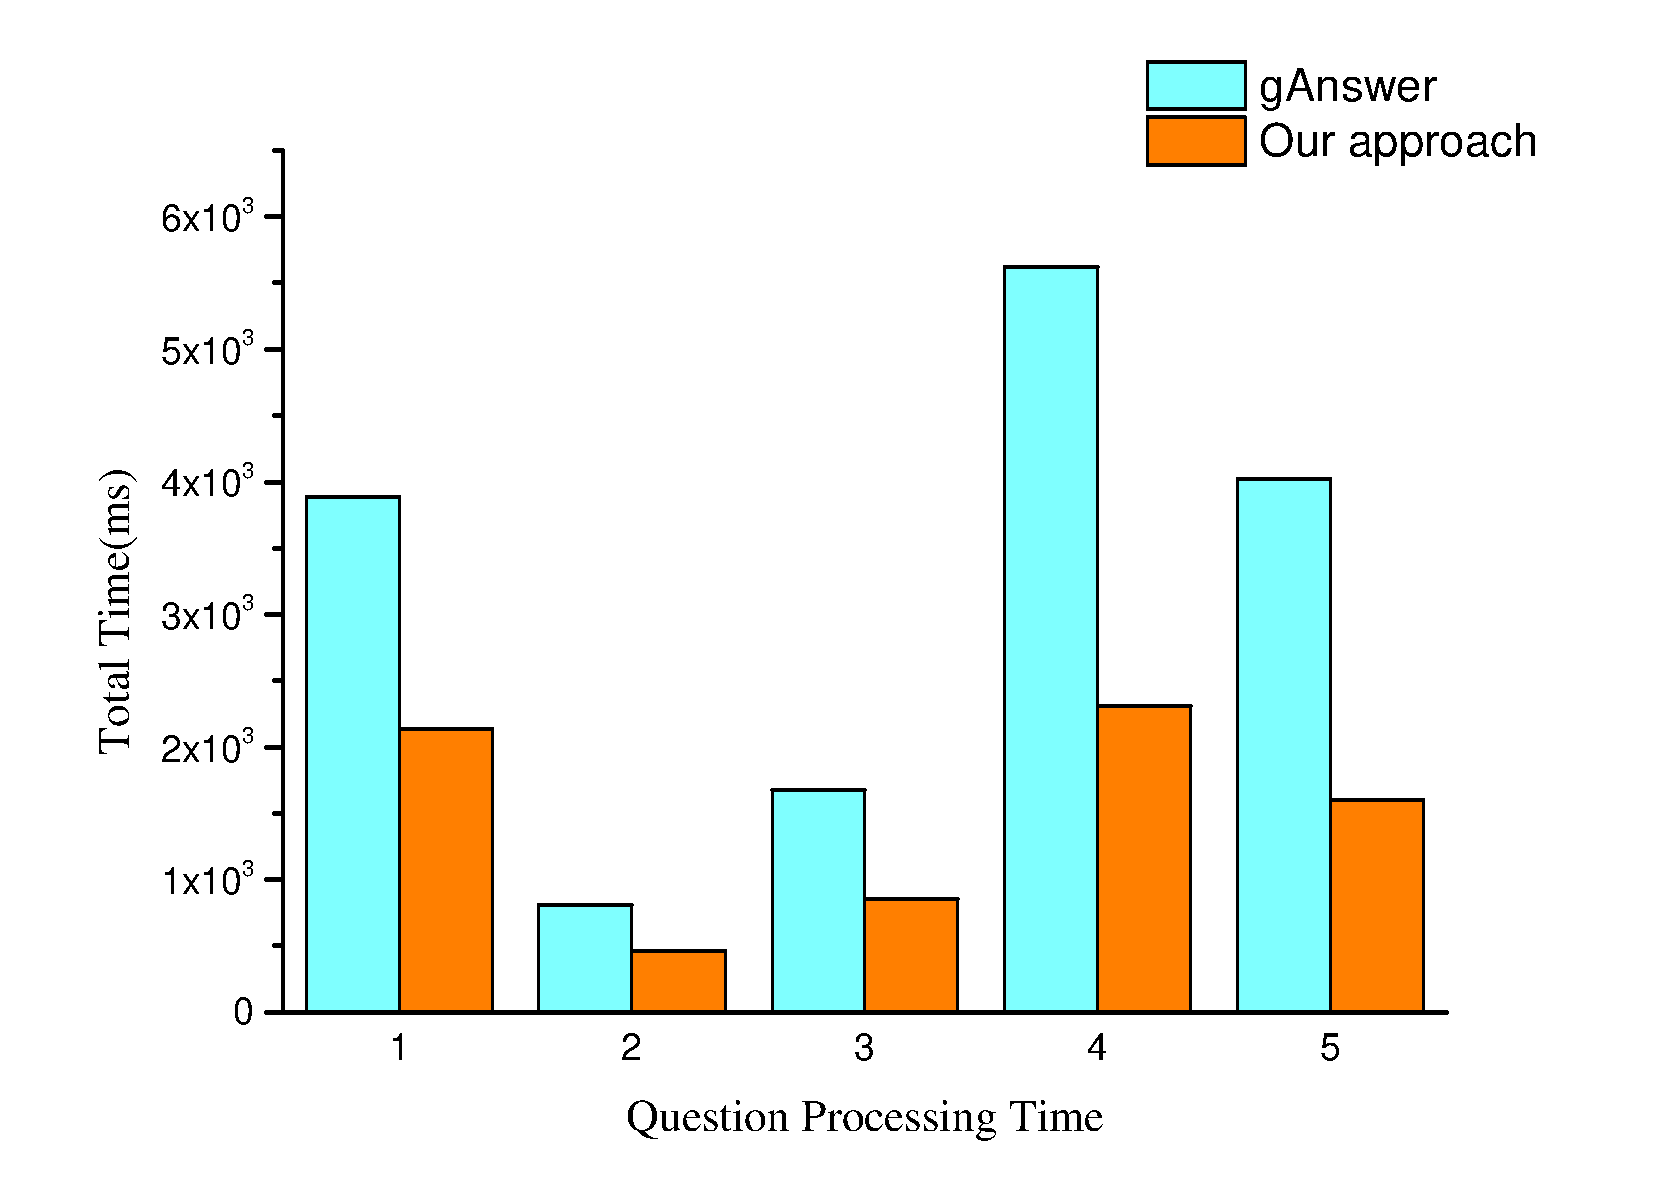
\includegraphics[width= 6cm]{QPT.pdf}
		\caption{Question processing time}
	\end{minipage}
	\begin{minipage}[t]{0.48\textwidth}
		\centering
		\label{fig3}
		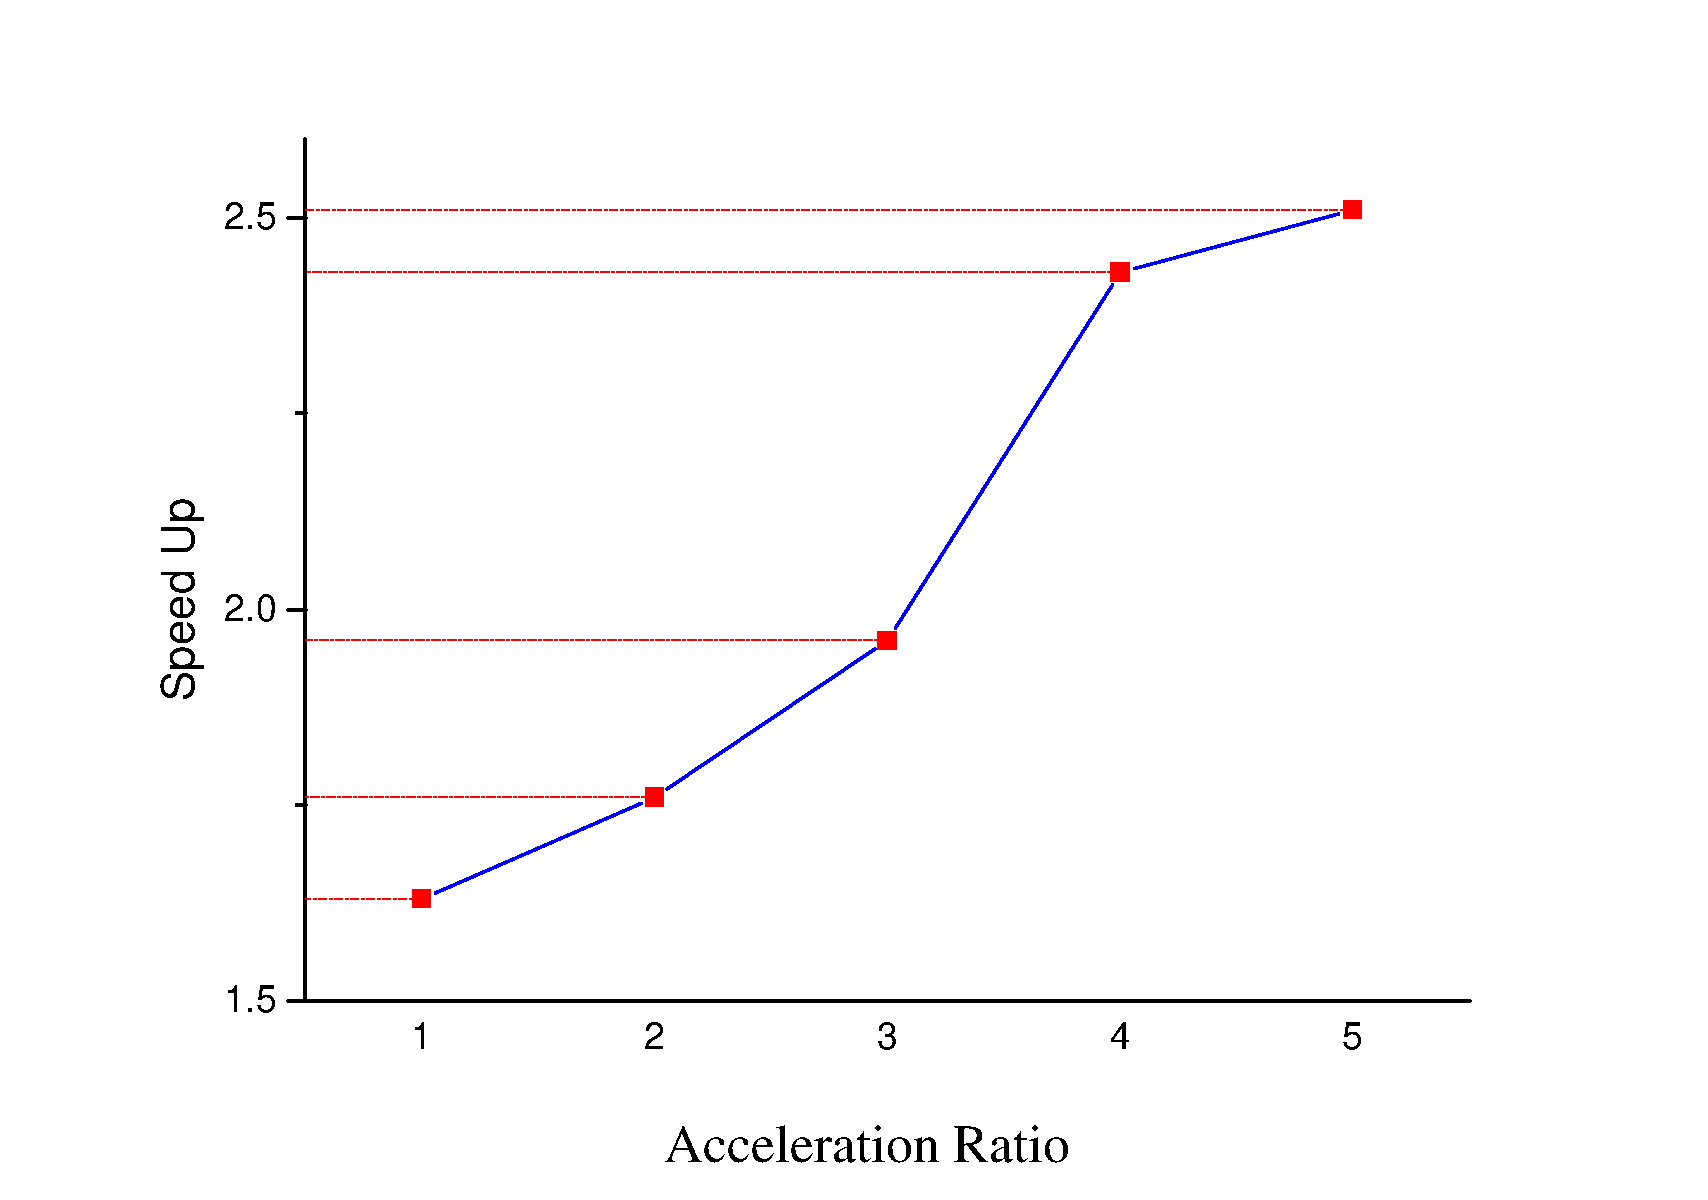
\includegraphics[width=6cm]{accelaration.pdf}
		\caption{Acceleration Ratio}
	\end{minipage}
\end{figure}

Figure 2 shows that by using our method, the RDF Q/A system greatly improves the efficiency of batch query processing with common structures. As shown in Figure \ref{fig3}, the efficiency is improved between 1.5 and 2.5 times. The rate of efficiency increase depends on the proportion of the entire structure occupied by the public structure. The greater the proportion of common structures, the more efficient it is.
% ---- Bibliography ----
%
% BibTeX users should specify bibliography style 'splncs04'.
% References will then be sorted and formatted in the correct style.
%
% \bibliographystyle{splncs04}
% \bibliography{mybibliography}
%
\begin{thebibliography}{8}
\bibitem{QAF}
James Bailey, Alistair Moffat, Charu~C. Aggarwal, Maarten de~Rijke, Ravi Kumar,
Vanessa Murdock, Timos~K. Sellis, and Jeffrey~Xu Yu, editors.
\newblock {\em  {CIKM} 2015, Melbourne, VIC, Australia,
	October 19 - 23, 2015}. {ACM}, 2015.

\bibitem{gAnswer}
Sen Hu, Lei Zou, Jeffrey~Xu Yu, Haixun Wang, and Dongyan Zhao.
\newblock Answering natural language questions by subgraph matching over
knowledge graphs (extended abstract).
\newblock In {\em 
	{ICDE} 2018, Paris, France, April 16-19, 2018}, pages 1815--1816, 2018.

\bibitem{RDF3X}
Thomas Neumann and Gerhard Weikum.
\newblock {RDF-3X:} a risc-style engine for {RDF}.
\newblock {\em {PVLDB}}.

\bibitem{junhu}
Xuguang Ren and Junhu Wang.
\newblock Multi-query optimization for subgraph isomorphism search.
\newblock {\em {PVLDB}}, 10(3):121--132, 2016.

\bibitem{gStore}
Lei Zou, M.~Tamer {\"{O}}zsu, Lei Chen, Xuchuan Shen, Ruizhe Huang, and Dongyan
Zhao.
\newblock gstore: a graph-based {SPARQL} query engine.
\newblock {\em {VLDB} J.}, 23(4):565--590, 2014.
\end{thebibliography}
\end{document}
